\documentclass[aspectratio=169, table]{beamer}

%\usepackage[beamertheme=./praditatheme]{Pradita}
\usepackage[utf8]{inputenc}

\usetheme{Pradita}

\subtitle{MTI102-Information Systems \&\\Technology Architecture}

\title{\huge Introduction to\\Enterprise Architecture}
\date[Serial]{\scriptsize {PRU/SPMI/FR-BM-18/0222}}
\author[Pradita]{\small {\textbf{Alfa Yohannis}}}

\begin{document}

    \frame{\titlepage}

    \begin{frame}
        \frametitle{Definition of 'Enterprise' According to }
        \framesubtitle{the Oxford English Dictionary}
        \begin{itemize}
            \item A project or undertaking, usually one that requires effort and courage.
            \item Initiative, dare to take risks to gain profits.
            \item Organization or business company.
        \end{itemize}
    \end{frame}

    \begin{frame}
        \frametitle{Definition of 'Enterprise' According to}
        \framesubtitle{the Cambridge English Dictionary}
        \begin{itemize}
            \item Ability to think about new plans and make them work.
            \item A company.
        \end{itemize}
    \end{frame}

    \begin{frame}
        \frametitle{Definition of 'Enterprise' According to}
        \framesubtitle{Merriam-Webster Dictionary}
        \begin{itemize}
            \item A project or endeavour that often requires courage.
            \item Readiness to engage in bold and risky ventures.
            \item An organized economic unit.
        \end{itemize}
    \end{frame}

    \begin{frame}
        \frametitle{Conclusion to the Definition}
        \framesubtitle{of `Enterprise'}
        \begin{itemize}
            \item 'Enterprise' refers to a bold, risky project or venture.
            \item Can also refer to an organization or business company.
            \item This definition is generally consistent among leading English dictionaries.
        \end{itemize}
    \end{frame}

    \begin{frame}
        \frametitle{Definition of 'Architecture' According to}
        \framesubtitle{the Oxford English Dictionary}
        \begin{itemize}
            \item The art or practice of designing and constructing buildings.
            \item Style or method of construction.
            \item The arrangement or structure of something.
        \end{itemize}
    \end{frame}

    \begin{frame}
        \frametitle{Definition of 'Architecture' According to}
        \framesubtitle{the Cambridge English Dictionary}
        \begin{itemize}
            \item The art and practice of designing buildings.
            \item The style or design of a specific building or group of buildings.
            \item The way something is done or arranged.
        \end{itemize}
    \end{frame}

    \begin{frame}
        \frametitle{Definition of 'Architecture' According to}
        \framesubtitle{Merriam-Webster Dictionary}
        \begin{itemize}
            \item The art or science of designing and constructing buildings.
            \item Method or style of construction.
            \item How the parts of something are arranged or systematized.
        \end{itemize}
    \end{frame}

    \begin{frame}
        \frametitle{Summary}
        \begin{itemize}
            \item 'Architecture' generally refers to the art or practice of designing and constructing buildings.
            \item Can also refer to a style or method of construction.
            \item Additionally, it can also refer to the way the parts of something are arranged or systematized.
        \end{itemize}
    \end{frame}

    \begin{frame}
        \frametitle{Definition of Architecture}
        \framesubtitle{according to IEEE}
        \begin{itemize}
            \item The fundamental organization of a system
            \item Involves system components, relationships between components
            \item Manages system design and evolution
            \item System components can include hardware, software, data, people, processes
        \end{itemize}
    \end{frame}



    \begin{frame}
        \frametitle{Definition of 'Enterprise Architecture'}
        \framesubtitle{According to Gartner}
        \begin{itemize}
            \item A discipline for project design, planning, implementation, and control.
            \item Helps organizations achieve business and IT consistency.
            \item Involves collaboration between various stakeholders.
            \item Can be used to assist in strategic decision-making.
        \end{itemize}
    \end{frame}

    \begin{frame}
        \frametitle{Definition of 'Enterprise Architecture'}
        \framesubtitle{According to TOGAF}
        \begin{itemize}
            \item An architectural framework.
            \item Provides a basic definition and design for enterprise architecture.
            \item Help ensure company operations run consistently and efficiently.
            \item Focuses on standards and procedures used within the company.
        \end{itemize}
    \end{frame}

    \begin{frame}
        \frametitle{Definition of 'Enterprise Architecture'}
        \framesubtitle{According to ISO/IEC/IEEE 42010}
        \begin{itemize}
            \item A fundamental approach to the organization of a system.
            \item Involves understanding all components, the relationships between components, and their environment.
            \item Emphasizes the importance of structure and interactions in systems.
            \item Provides a framework for systems understanding and design.
        \end{itemize}
    \end{frame}



    \begin{frame}
        \frametitle{Various Enterprise Architecture Frameworks}
        \framesubtitle{\hspace{1cm}}
        \begin{itemize}
            \item Business System Planning (BSP)
            \item PRISM Architecture Framework
            \item NIST Enterprise Architecture Model
            \item Zachman Framework
            \item EAP: Enterprise Architecture Planning
            \item Sherwood Applied Business Security Architecture
            \item Federal Enterprise Architecture Framework

        \end{itemize}

    \end{frame}
    \begin{frame}
        \frametitle{Various Enterprise Architecture Frameworks (2)}
        \framesubtitle{\hspace{1cm}}
        \begin{itemize}
            \item Gartner's Enterprise Architecture Method
            \item Department of Defense Architecture Framework (DoDAF)
            \item Australian Government AGA
            \item Business Architecture Body of Knowledge (BizBoK)
            \item ISO Standard for Enterprise Modeling (ISO19439)
        \end{itemize}
    \end{frame}

    \begin{frame}
        \frametitle{Business System Planning}
        \begin{itemize}
            \item This process involves understanding business goals, analyzing business processes, and designing an information system architecture that supports these processes.
            \item BSP helps organizations improve efficiency, simplify operations, and optimize resource allocation.
        \end{itemize}
    \end{frame}

    {
        \setbeamertemplate{navigation symbols}{}
        \setbeamertemplate{footline}{}
        \begin{frame}
            \frametitle{Business System Planning (BSP)}
            \begin{center}
                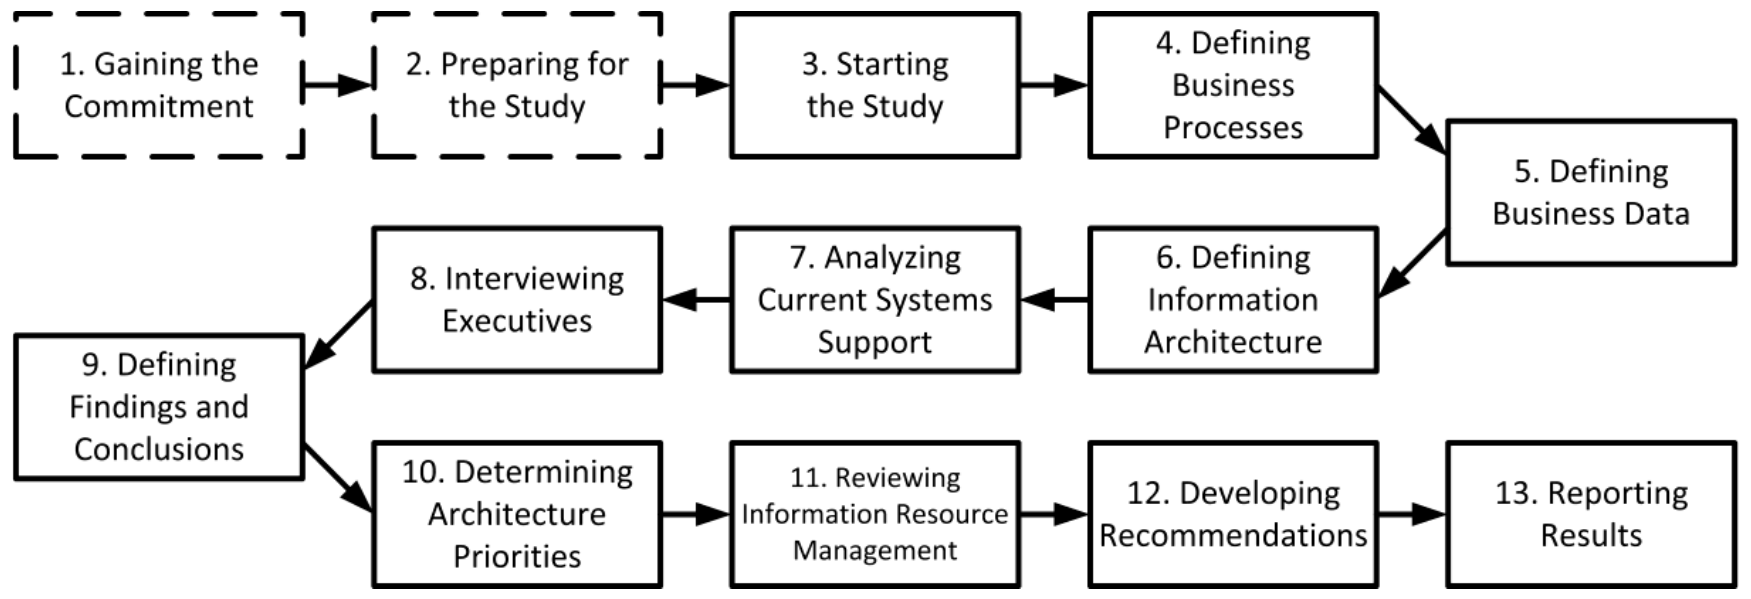
\includegraphics[width=\textwidth]{../figures/bsp}
            \end{center}
        \end{frame}
    }

    \begin{frame}
        \frametitle{PRISM Architecture Framework}
%        \framesubtitle{\hspace{1cm}}
        \begin{itemize}
            \item \textbf{Partnership for Research in Information Systems Management}
            \item One of the first enterprise architecture frameworks
            \item Developed by a consortium of IT vendors
            \item Focuses on system integration and information technology
            \item Helps organizations understand and manage IT complexity
        \end{itemize}
    \end{frame}

    {
        \setbeamertemplate{navigation symbols}{}
        \setbeamertemplate{footline}{}
        \begin{frame}
            \frametitle{PRISM Architecture Framework}
%            \framesubtitle{\hspace{1cm}}
            \begin{center}

                \begin{figure}[ht]
                    \begin{minipage}[b]{0.49\linewidth}
                        \centering
                        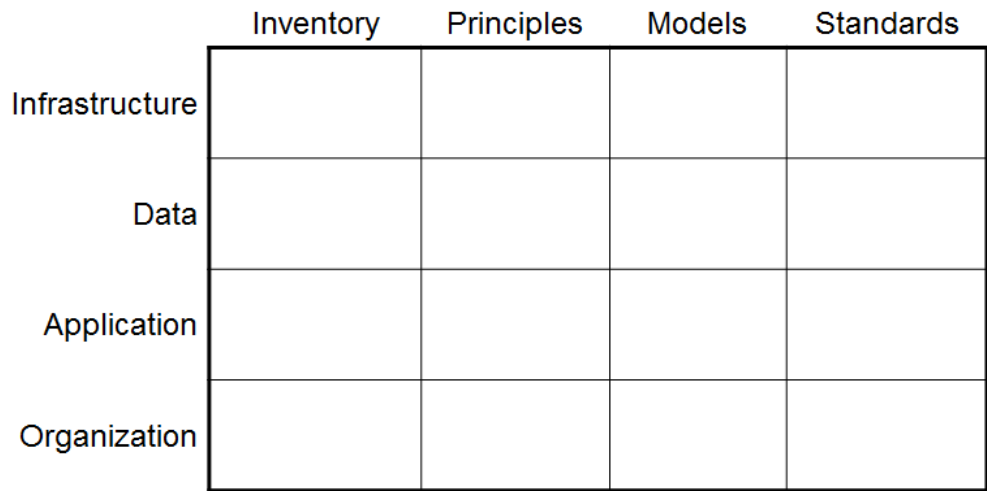
\includegraphics[width=\textwidth]{../figures/prism_matrix}
                        \caption{matrix}
                    \end{minipage}
                    \hfill
                    \begin{minipage}[b]{0.49\linewidth}
                        \centering
                        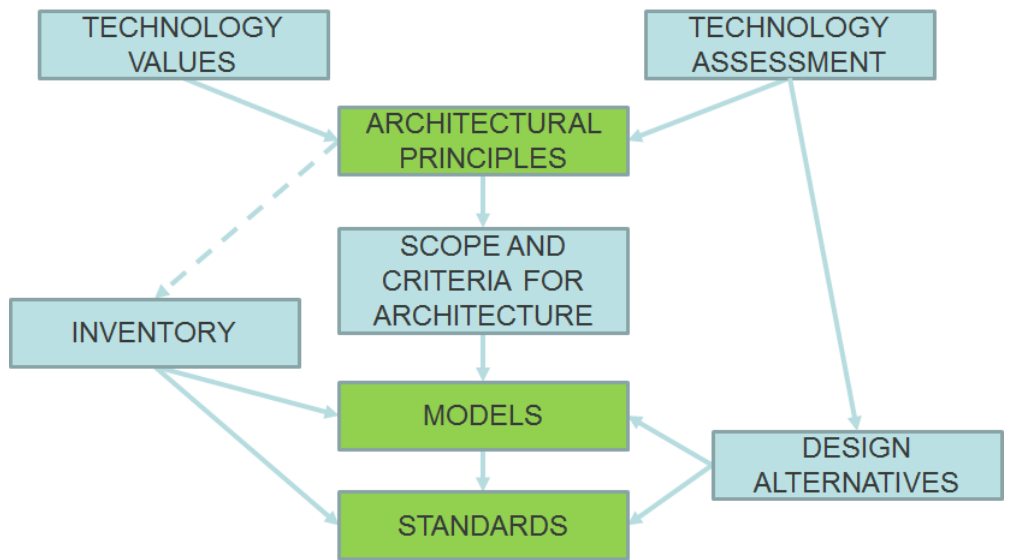
\includegraphics[width=\textwidth]{../figures/prism_relationships}
                        \caption{relationships}
                    \end{minipage}
                \end{figure}

            \end{center}
        \end{frame}
    }

    \begin{frame}
        \frametitle{NIST Enterprise Architecture Model}
        \framesubtitle{\hspace{1cm}}
        \begin{itemize}
            \item  \textbf{National Institute of Standards and Technology}
            \item Emphasizes structuring and organizing IT operations
            \item Divides IT architecture into five levels
            \item Focuses on business, data, applications, technology and results
            \item Enables strategic planning and data-driven decision-making
        \end{itemize}
    \end{frame}

    {
        \setbeamertemplate{navigation symbols}{}
        \setbeamertemplate{footline}{}
        \begin{frame}
            \frametitle{NIST Enterprise Architecture Framework}
            \framesubtitle{\hspace{1cm}}
            \begin{center}
                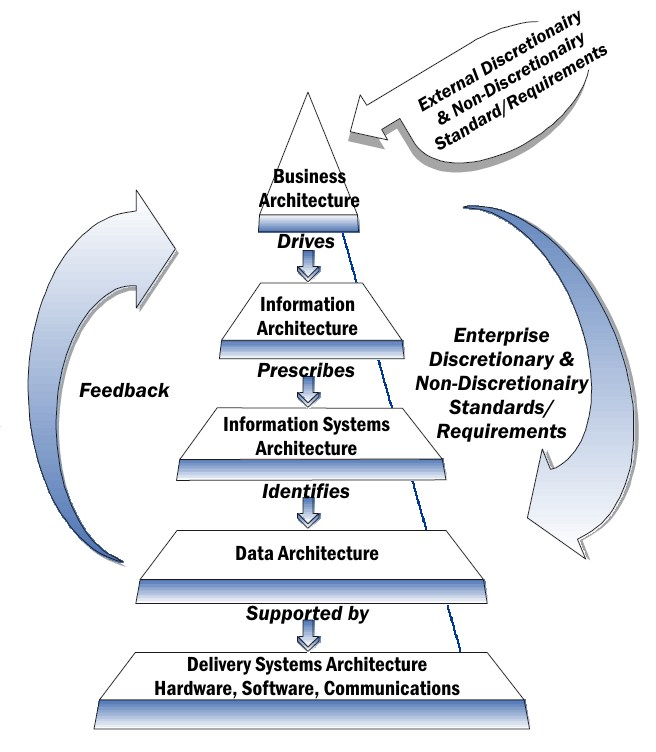
\includegraphics[width=.40\textwidth]{../figures/nist}
            \end{center}
        \end{frame}
    }

    \begin{frame}
        \frametitle{Zachman Framework}
        \begin{itemize}
            \item A schema for understanding and managing the complexity of enterprise architecture
            \item Divided into six different levels
            \item Summarize from the most abstract to the most concrete level
            \item Suitable for many types of organizations, from business to government
        \end{itemize}
    \end{frame}

    {
        \setbeamertemplate{navigation symbols}{}
        \setbeamertemplate{footline}{}
        \begin{frame}
            \frametitle{Zachman Framework}
             \framesubtitle{\hspace{1cm}}
            \vspace{10pt}
            \begin{center}
                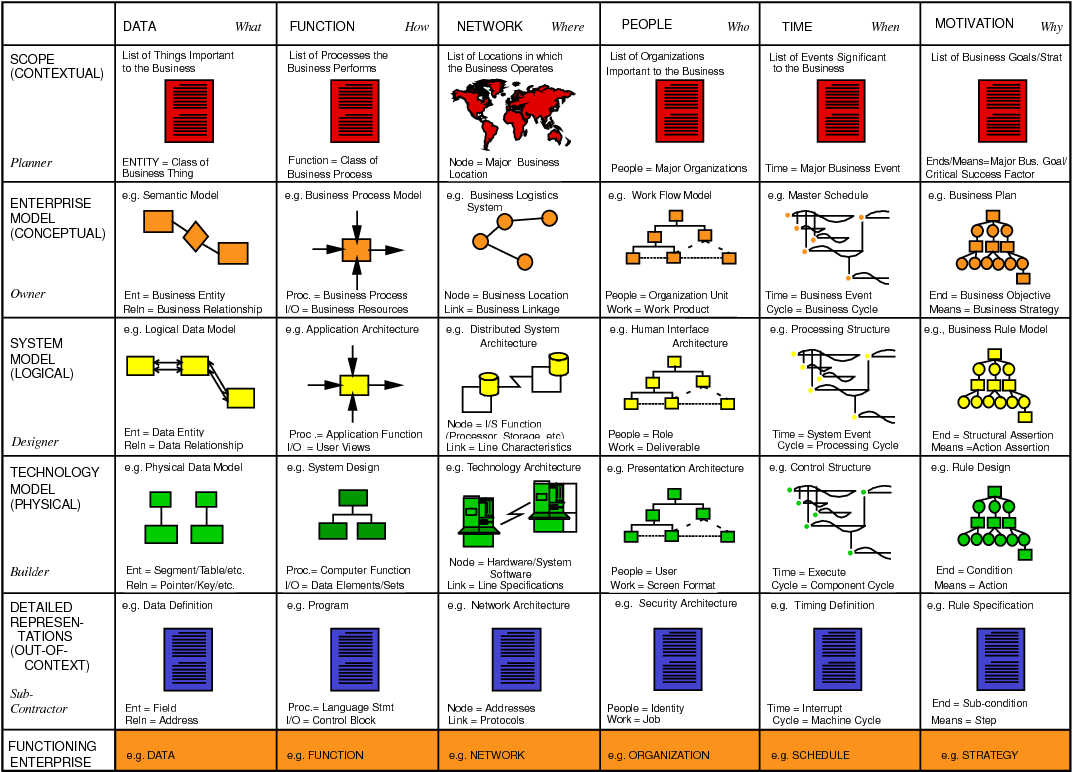
\includegraphics[width=0.76\textwidth]{../figures/zachman}
            \end{center}
        \end{frame}
    }

    \begin{frame}
        \frametitle{Enterprise Architecture Planning (EAP)}
        \framesubtitle{\hspace{1cm}}
        \begin{itemize}
            \item Methods for planning information systems architecture
            \item Identify what the business needs from information technology
            \item Develop plans for implementation of new technology based on business needs
            \item Can help in digital transformation and organizational change
        \end{itemize}
    \end{frame}

    {
        \setbeamertemplate{navigation symbols}{}
        \setbeamertemplate{footline}{}
        \begin{frame}
            \frametitle{Enterprise Architecture Planning}
            \begin{center}
                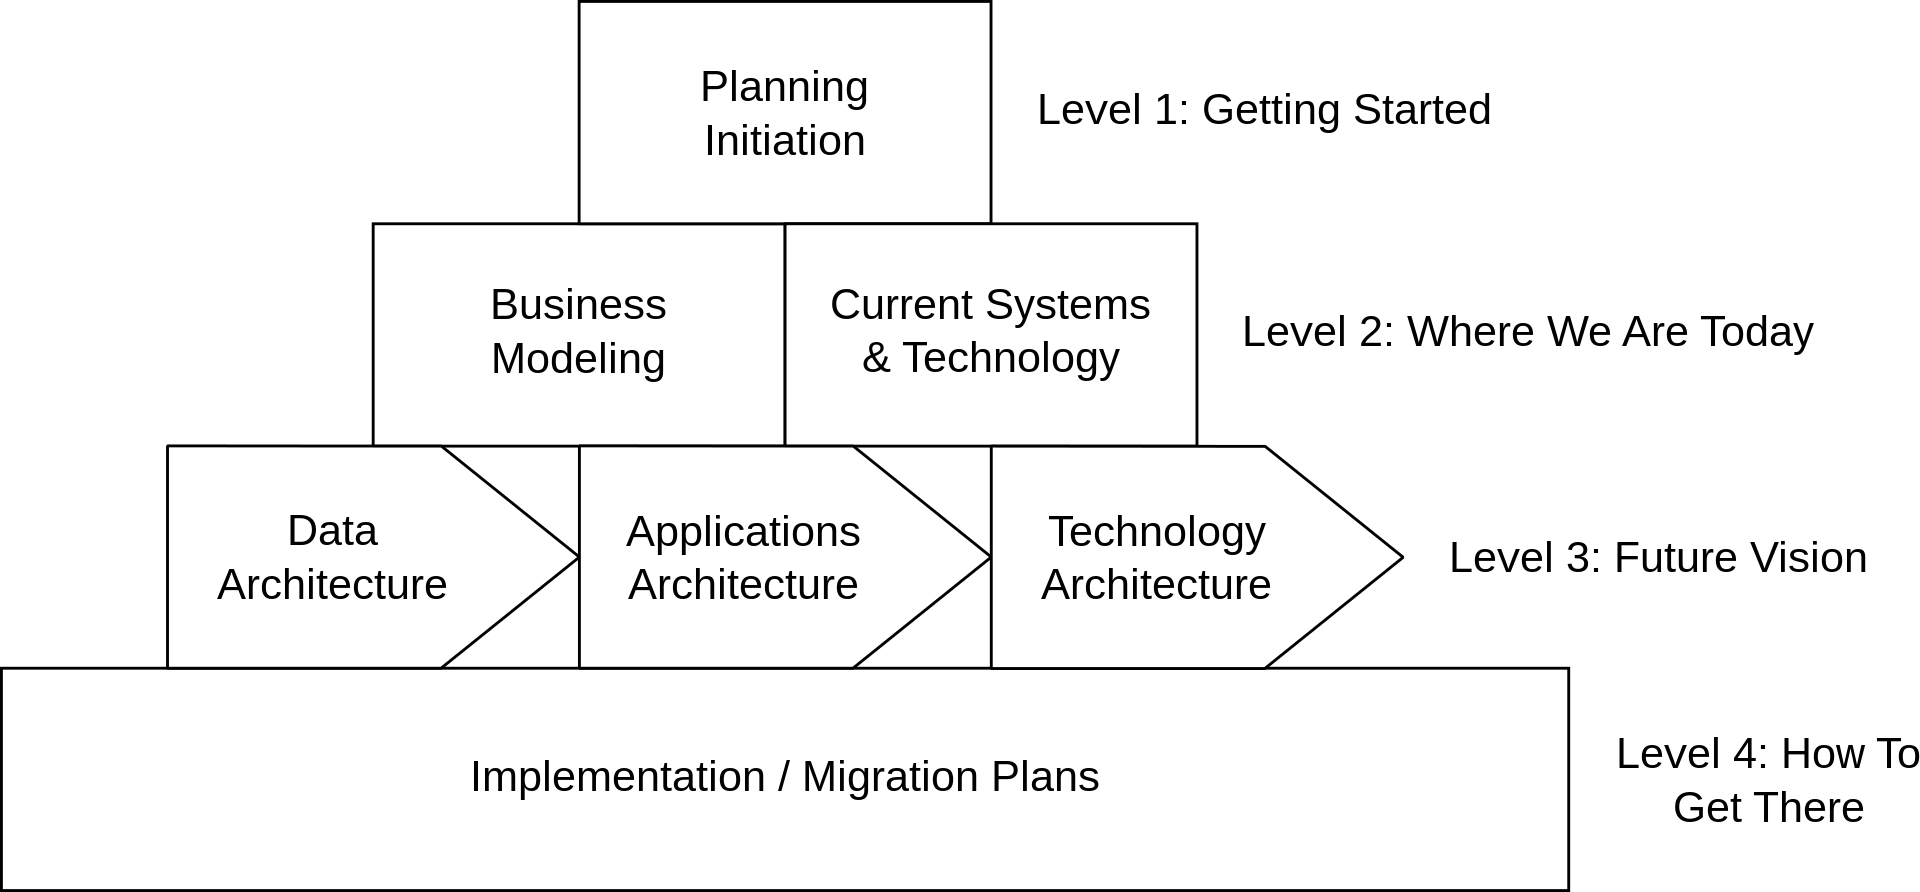
\includegraphics[width=1\textwidth]{../figures/eap}
            \end{center}
        \end{frame}
    }

    \begin{frame}
        \frametitle{Sherwood Applied Business Security Architecture (SABSA)}
        \framesubtitle{\hspace{1cm}}
        \begin{itemize}
            \item Models and methodologies for developing information security and risk management frameworks
            \item Design, implement, and manage business-centric security solutions
            \item Developed with a "start-to-finish" and "top-down" approach
            \item Can be tailored to the specific needs of the organization
        \end{itemize}
    \end{frame}

    {
        \setbeamertemplate{navigation symbols}{}
        \setbeamertemplate{footline}{}
        \begin{frame}
            \frametitle{Sherwood Applied Business Security Architecture (SABSA)}
            \framesubtitle{\hspace{1cm}}
            \begin{center}
                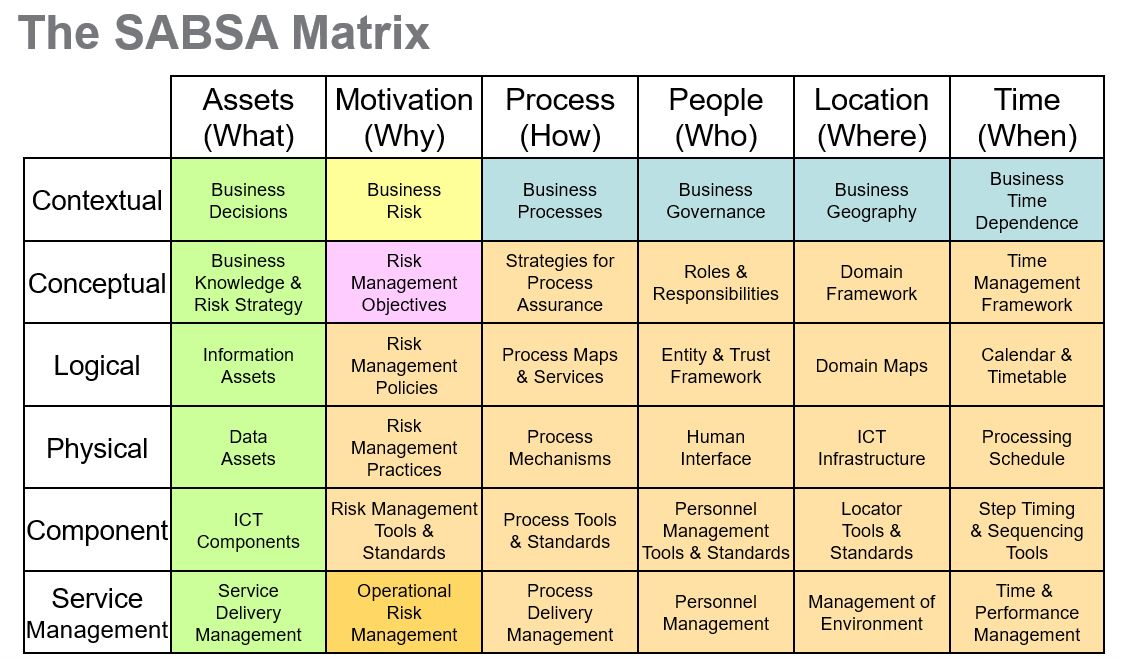
\includegraphics[width=0.8\textwidth]{../figures/sabsa}
            \end{center}
        \end{frame}
    }


    \begin{frame}
        \frametitle{Federal Enterprise Architecture Framework (FEAF)}
        \framesubtitle{\hspace{1cm}}
        \begin{itemize}
            \item Framework used by the US federal government
            \item Helps in improving the efficiency and effectiveness of government services
            \item Facilitate collaboration between government agencies and departments
            \item Is part of the US government's information technology modernization strategy
        \end{itemize}
    \end{frame}

    {
        \setbeamertemplate{navigation symbols}{}
        \setbeamertemplate{footline}{}
        \begin{frame}
            \frametitle{Federal Enterprise Architecture Framework}
            \framesubtitle{\hspace{1cm}}
            \begin{center}
                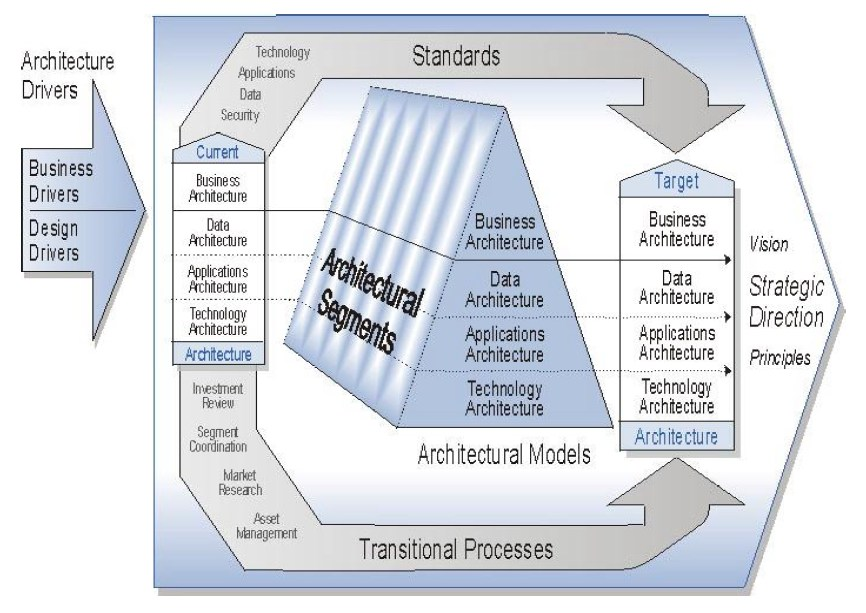
\includegraphics[width=.75\textwidth]{../figures/feaf}
            \end{center}
        \end{frame}
    }

    \begin{frame}
        \frametitle{Gartner Enterprise Architecture Method}
        \framesubtitle{\hspace{1cm}}
        \begin{itemize}
            \item Method developed by the research and consulting company Gartner
            \item Guide organizations in designing, developing, and implementing enterprise architecture
            \item Linking business strategy and IT
            \item Help organizations achieve digital transformation goals
        \end{itemize}
    \end{frame}

    {
        \setbeamertemplate{navigation symbols}{}
        \setbeamertemplate{footline}{}
        \begin{frame}
            \frametitle{Gartner's Enterprise Architecture Process}
            \framesubtitle{\hspace{1cm}}
            \begin{center}
                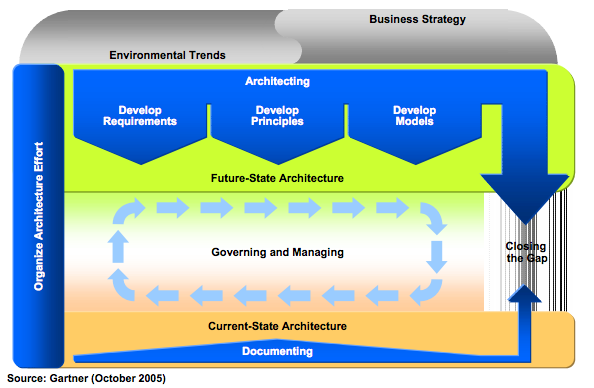
\includegraphics[width=.70\textwidth]{../figures/gartner}
            \end{center}
        \end{frame}
    }

    \begin{frame}
        \frametitle{Department of Defense Architectural Framework (DoDAF)}
        \framesubtitle{\hspace{1cm}}
        \begin{itemize}
            \item Framework used by the US Department of Defense
            \item Helps in organizing and visualizing information important to the decision-making process
            \item Uses various models and guides to develop architecture
            \item Suitable for organizations of large complexity and scale
        \end{itemize}
    \end{frame}

    {
        \setbeamertemplate{navigation symbols}{}
        \setbeamertemplate{footline}{}
        \begin{frame}
            \frametitle{Department of Defense Architecture Framework (DoDAF)}
            \framesubtitle{\hspace{1cm}}
            \begin{center}
                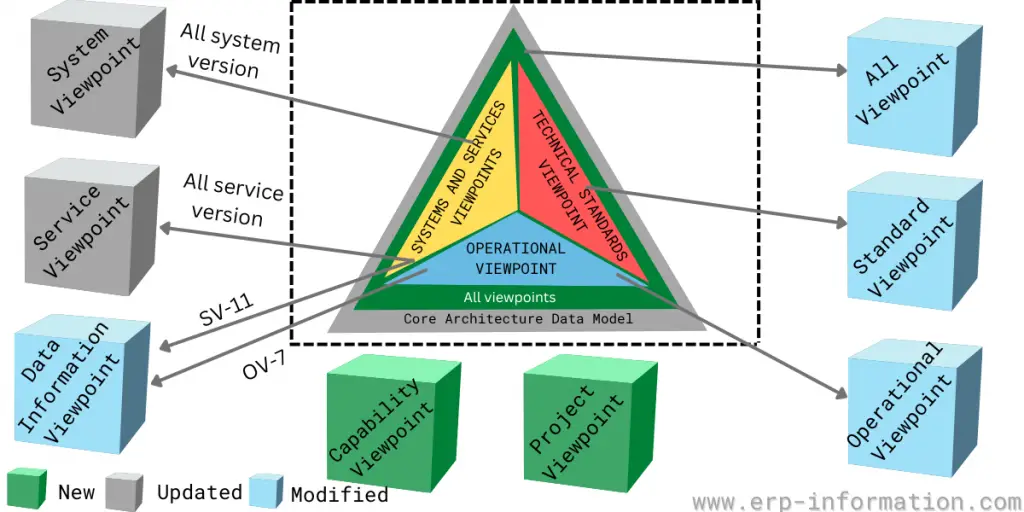
\includegraphics[width=0.68\textwidth]{../figures/dodaf}
            \end{center}
        \end{frame}
    }

    \begin{frame}
        \frametitle{Australian Government AGA}
        \begin{itemize}
            \item Framework used by the Australian Government
            \item Assist in the planning and implementation of information technology at the government level
            \item Encourage collaboration between government departments and agencies
            \item Increase efficiency and transparency in government services
        \end{itemize}
    \end{frame}

    {
        \setbeamertemplate{navigation symbols}{}
        \setbeamertemplate{footline}{}
        \begin{frame}
            \frametitle{Austarlian Government Architecture (AGA)}
            \framesubtitle{\hspace{1cm}}
            \begin{center}
                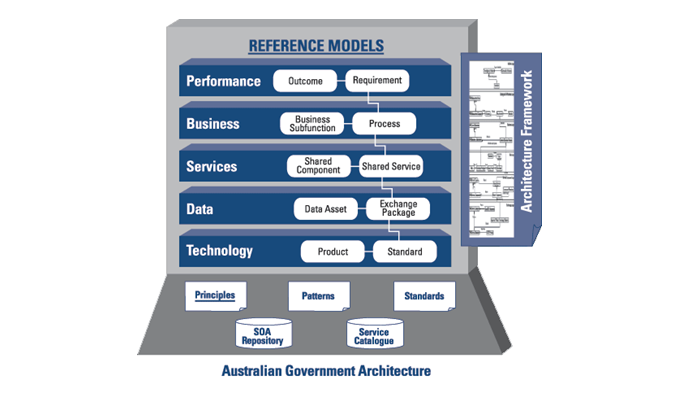
\includegraphics[width=0.9\textwidth]{../figures/aga}
            \end{center}
        \end{frame}
    }

    \begin{frame}
        \frametitle{Business Architecture Body of Knowledge (BizBoK)}
        \framesubtitle{\hspace{1cm}}
        \begin{itemize}
            \item Guide developed by the Business Architecture Guild
            \item Provides best practices and standards in business architecture
            \item Can be used by business architects and other related professionals
            \item Helps organizations in designing and implementing business architecture
        \end{itemize}
    \end{frame}

    {
        \setbeamertemplate{navigation symbols}{}
        \setbeamertemplate{footline}{}
        \begin{frame}
            \frametitle{Business Architecture Body Of Knowledge}
            \framesubtitle{\hspace{1cm}}
            \begin{center}
                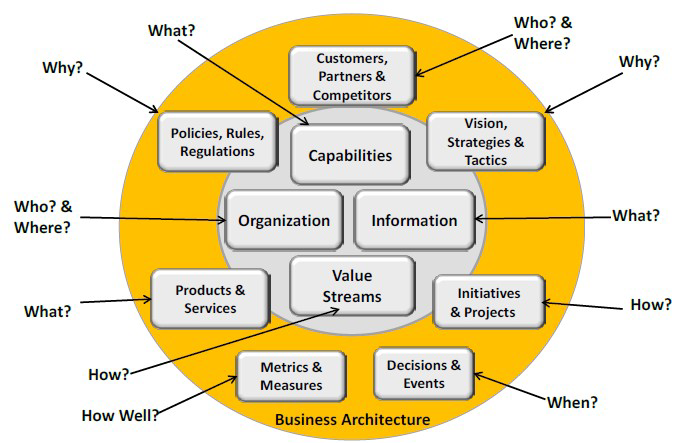
\includegraphics[width=0.7\textwidth]{../figures/bizbok}
            \end{center}
        \end{frame}
    }

    \begin{frame}
        \frametitle{ISO Standard for Enterprise Modeling (ISO19439)}
        \framesubtitle{\hspace{1cm}}
        \begin{itemize}
            \item International standard for modelling business and organizational processes
            \item Assists in planning, design, and improvement of business processes
            \item Can be used by many types of organizations, from business to government
            \item Developed by the International Organization for Standardization (ISO)
        \end{itemize}
    \end{frame}

    {
        \setbeamertemplate{navigation symbols}{}
        \setbeamertemplate{footline}{}
        \begin{frame}
            \frametitle{ISO19439 Enterprise Modelling}
            \begin{center}
                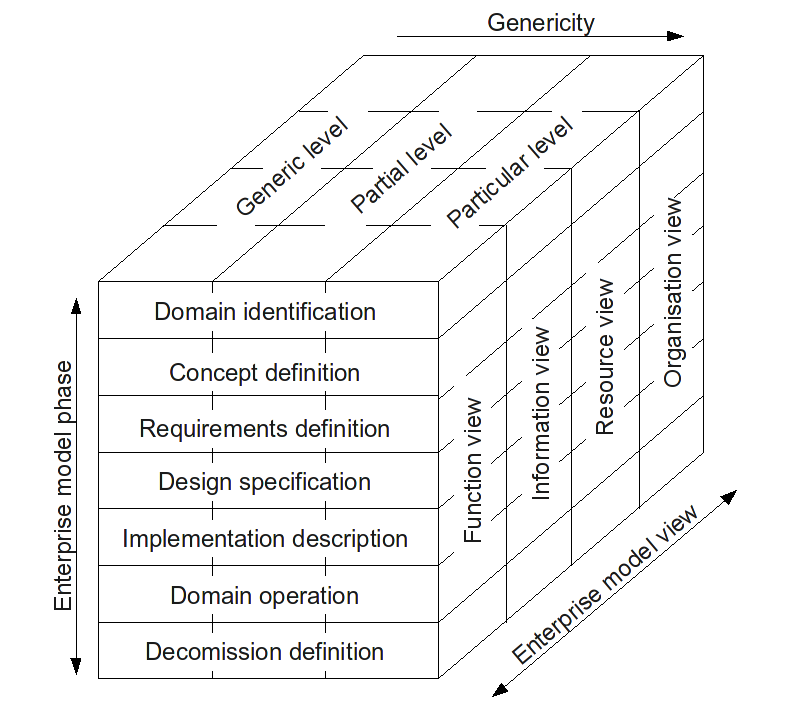
\includegraphics[width=.45\textwidth]{../figures/iso19439}
            \end{center}
        \end{frame}
    }

    \begin{frame}
        \frametitle{Summary}
        \begin{itemize}
            \item There are various enterprise architecture frameworks and methodologies
            \item The choice of framework or methodology depends on the organization's specific needs and context
            \item Enterprise architecture is an important tool for planning and managing information technology in organizations
        \end{itemize}
    \end{frame}

\end{document}